\begin{refsection}

\begin{figure}
\begin{center}
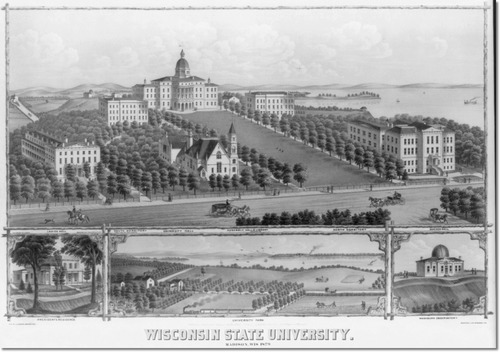
\includegraphics[width=.9\textwidth,trim=0 30 10 2, clip=true]{../pictures/wisconsin-map.jpg}
\end{center}
\vspace{-.2cm}
\caption{A prototypical university.  Caption reads: ``Wisconsin State
  University, Madison, Wis. 1879''.  Inset captions describe the
  pictured buildings: ``Ladies Hall, South Dormitory, University Hall,
  Assembly Halls \& Library, North Dormitory, Science Hall, President's
  Residence, University Farm, and Washburn Observatory.''  Public
  domain.\label{madison-map}}
\end{figure}

This chapter outlines an approach to the organization of learning that draws on the principles of free\slash libre\slash open source software (FLOSS), free culture, and peer production.
Mako Hill suggests that one recipe for success in peer production is to take a familiar idea -- for example, an encyclopedia -- and make it easy for people to participate in building it \cite[Chapter 1]{mako-thesis}.  We will take hold of ``learning in institutions'' as a map (Figure \ref{madison-map}), although it does not fully conform to our chosen tacitly-familiar territory of \emph{peeragogy}.  To be clear, peeragogy is for \emph{any group of people who want to learn anything}.\footnote{\url{https://www.youtube.com/watch?v=TDRGJzoNbAc}}
 

Despite thinking about learning and adaptation that
may take place far outside of formal institutions, the historical
conception of a university helps give shape to our inqury.
%
The model university is not separate from the life of the state or its
citizenry, but aims to ``assume leadership in the application of
knowledge for the direct improvement of the life of the people in
every sphere'' \cite[p.~88]{curti1949university}. Research that
\emph{adds to the store of knowledge} is another fundamental
obligation of the university \cite[p.~550]{curti1949university}.
The university provides a familiar model for collaborative knowledge work
but it is not the only model available.
% wording issues here
Considering the role of collaboration in building Wikipedia,
StackExchange, and free\slash libre\slash open source software
development, we may be led to ask:  What might an accredited free\slash
libre\slash open university look like?  How would it compare or
contrast with the typical or stereotypical image of a university from
Figure \ref{madison-map}?  Would it have similar structural features, like a Library,
Dormitory, Science Hall and so on?  Would participants take
on familiar roles \cite{corneli+crowdsourcing}?  How would it compare
with historical efforts like the Tuskegee Institute that involved
students directly in the production of physical infrastructure
\cite{washington1986up,building-peeragogy-accelerator}?
%
We use the word \emph{peeragogy} to talk about collaboration in
relatively non-hierarchical settings.  Examples are found in
education, but also in business, government, volunteer, and NGO
settings.  Peeragogy involves both problem solving and problem
definition.  Indeed, in many cases it is preferable to focus on
solutions, since people know the ``problems'' all too well
\cite{ariyaratneXorganizationX1977}.  Participants in a peeragogical
endeavor collaboratively build emergent structures that are responsive
to their changing context, and that in turn, change that context. In
the Peeragogy project, we are developing the the theory and practice
of peeragogy.

\emph{Design patterns} offer a methodological framework that we have
used to clarify our focus and organize our work.  A design pattern
expresses a commonly-occurring problem, a solution to that problem,
and rationale for choosing this solution \cite{meszaros1998pattern}.
This skeleton is typically fleshed out with a \emph{pattern template}
that includes additional supporting material; individual patterns are
connected with each other in a \emph{pattern language}.  What we
present here is rather different from previous pattern languages that touch
on similar topics -- like \emph{Liberating Voices}
\cite{schuler2008liberating}, \emph{Pedagogical Patterns}
\cite{bergin2012pedagogical}, and \emph{Learning Patterns}
\cite{iba2014learning}.  At the level of the pattern template, our
innovation is simply to add a ``What's next'' annotation, which
anticipates the way the pattern will continue to ``resolve''.

% The patterns we introduce here focus on negotiating the execution and implementation of solutions in their practical context.
%  This often requires compromise, adjustments and even restarts.  

This addition mirrors the central considerations of our approach, which is all about human interaction, and the challenges, fluidity and unpredictability that come with it.  Something that works for one person may not work for another or may not even work for the same person in a slightly different situation.  We need to be ready to clarify and adjust what we do as we go.   Even so, it is hard to argue with a sensible-sounding formula like ``If W applies, do X to get Y.'' In our view, other pattern languages often achieve this sort of common sense rationality, and then stop.  Failure in the prescriptive model only begins when people try to define things more carefully and make context-specific changes -- when they actually try to put ideas into practice.  The problem lies in the inevitable distance between \emph{do as I say}, \emph{do as I do}, and \emph{do with me} \cite[p.~26]{deleuze1994difference}.
%One is put in mind of Alfred Korzybski's famous remark: ``the map is not the territory.''   
%% Indeed, the strong version of our claim is that peeragogy is needed in applications of any map, blueprint, or design that seeks to involve people as people.
%% In some idealized sense, according to a certain school of thought, ``control'' is all that's required to move from a well-thought-out design to successful execution.  But, where do the designs come from in the first place \cite{von2003cybernetics}?
%% %
%% Moreover, once they exist, designs need to be interpreted, and often, revised.  
If people are involved, things get messy.   They may think that they are on the same page, only to find out that their understandings are wildly different.  For  example, everyone may agree that the group needs to go ``that way.''  But how far?  How fast?  It is rare for a project to be able to set or even define all of the parameters accurately and concisely at the beginning.
And yet design becomes a ``living language'' \cite[p.~xvii]{alexander1977pattern}  just insofar as it is linked to action.  Many things have changed since Alexander suggested that ``you will get the most `power' over the language, and make it your own most effectively, if you write the changes in, at the appropriate places in the book'' \cite[p.~xl]{alexander1977pattern}.  We see more clearly what it means to inscribe the changing form of design not just in the margins of a book, or even a shared wiki, but in the lifeworld itself.  Other recent authors on patterns share similar views \cite{reiners2012approach, plast-project, schummer2014beyond}.


%% We use the patterns of peeragogy to
%% \emph{constitute and occupy practical or speculative problems as such}
%% \cite[p.~204]{deleuze1994difference}.
%% %
%% Our patterns are a living language just insofar as they are linked to
%% action.

% Till Sch{\"u}mmer \emph{et al.}~have emphasized that pattern authors ``talk about what by definition is tacit'' and highlight the role of nonverbal communication ``needed to communicate the unspeakable'' \cite[p.~9]{schummer2014beyond}.

%% Whereas existing projects like Wikimedia's Wikiversity\footnote{\url{https://www.wikiversity.org/}} and the Peer-2-Peer University (P2PU) have created ``a model for lifelong learning alongside traditional formal higher education,''\footnote{\url{https://www.p2pu.org/en/}} they stop well short of offering accredited degrees.  

Learning and collaboration are of interest to both organizational studies and computer science, where researchers are increasingly making use of social approaches to software design and development, as well as agent-based models of computation \cite{minsky1967programming,poetry-workshop}.
%
The design pattern community in particular is very familiar with practices that we think of as peeragogical, including shepherding, writers workshops, and design patterns themselves \cite{harrison1999language,coplien1997pattern,meszaros1998pattern}.  %% We hope to help design pattern authors and researchers expand on these strengths.

\subsection*{Pattern template}

%This section will give the reader a sense of how the paper is organized. 


%% \begin{wraptable}{r}{.52\textwidth}
%% {\small

%% \begin{tabular}{|p{.5\textwidth}|}
%% \hline
%% \emph{Motivation} for using this pattern.\\ \hline
%% \end{tabular}
%% \vspace{-.1cm}

%% \begin{tabular}{|p{.5\textwidth}|}
%% \hline
%% \emph{Context} of application.\\ \hline
%% \emph{Forces} that operate within the context of application, each with a mnemonic glyph. \\ \hline
%% \emph{Problem} the pattern addresses.\\ \hline
%% \emph{Solution} to the problem.\\ \hline
%% \emph{Rationale} for this solution.\\ \hline
%% \emph{Resolution} of the forces, named in bold.\\ \hline
%% \end{tabular}
%% \vspace{.1cm}

%% %% \begin{tabular}{|p{.5\textwidth}|}
%% %% \hline
%% %% \emph{Inversion} Problems that could arise, and when \emph{not} to use the pattern.\\ \hline
%% %% \end{tabular}
%% %% \vspace{.1cm}

%% \begin{tabular}{|p{.5\textwidth}|}
%% \hline
%% \emph{Example 1}: How the pattern manifests in current Wikimedia projects.\\ \hline
%% \emph{Example 2}: How the pattern could inform the design of a future university.\\ \hline
%% \end{tabular}
%% \vspace{.1cm}

%% \begin{tabular}{|p{.5\textwidth}|}
%% \hline
%% \emph{What's Next in the Peeragogy Project}: How the pattern relates to our collective intention in the Peeragogy project\\ \hline
%% \end{tabular}

%% \vspace{-.1cm}
%% \caption{Pattern template.\label{tab:pattern-template}}
%% \vspace{-.9cm}
%% }
%% \end{wraptable}

Table \ref{tab:pattern-template} shows the pattern template that we use to present our patterns.
Along with the traditional design patterns components \cite{meszaros1998pattern}, each of our patterns is fleshed out with two illustrative examples.  The first is descriptive, and looks at how the pattern applies in current Wikimedia projects.  We selected Wikimedia as a source of examples because the project is familiar, a demonstrated success, and readily accessible.  The second example shows how the pattern could be applied in the design of a future university.  Each pattern concludes with a boxed annotation: ``\emph{What's Next in the Peeragogy Project}''.

%% Section \ref{sec:Peeragogy} defines the concept of \patternname{Peeragogy} more explicitly the form of a design pattern.  Sections \ref{sec:Roadmap}--\ref{sec:Scrapbook} present the other patterns in our pattern language. Figure \ref{fig:connections} illustrates their interconnections. Table \ref{tab:core} summarizes the ``nuts and bolts'' of the pattern language.
%% Section \ref{sec:Distributed_Roadmap} collects our ``What's Next'' steps, summarizes the outlook of the Peeragogy project.

%OSS: who cares? start w/example?
\subsection*{A short motivating example}
When one relative \patternname{Newcomer} was still in the onboarding
process in Peeragogy project, she hit a wall in understanding the
``patterns'' section in the \emph{Peeragogy Handbook} v1.  A more
seasoned peer invited her to a series of separate discussions with
their own \patternname{Heartbeat} to flesh out the patterns and make
them more accessible.  At that time the list of patterns was simply a
list of paragraphs describing recurrent trends.  During those
sessions, the impact and meaning of patterns captured her imagination.
She went on to become the champion for the pattern language and its
application in the Peeragogy project.  During a ``hive editing''
session, she proposed the template we initially used to give structure
to the patterns.  She helped further revise the pattern language for
the \emph{Peeragogy Handbook} v3, and attended PLoP 2015.  While a new
domain can easily be overwhelming, this newcomer found \patternname{A
  specific project} to start with, and scaffolded her knowledge and
contributions from that foundation.

\begin{table}
{\centering
\vspace{-.65cm}
\begin{tabular}{|p{.5\textwidth}|}
\hline
\emph{Motivation} for using this pattern.\\ \hline
\end{tabular}
\vspace{.1cm}

\begin{tabular}{|p{.5\textwidth}|}
\hline
\emph{Context} of application.\\ \hline
\emph{Forces} that operate within the context of application, each with a mnemonic glyph. \\ \hline
\emph{Problem} the pattern addresses.\\ \hline
\emph{Solution} to the problem.\\ \hline
\emph{Rationale} for this solution.\\ \hline
\emph{Resolution} of the forces, named in bold.\\ \hline
\end{tabular}
\vspace{.1cm}

%% \begin{tabular}{|p{.5\textwidth}|}
%% \hline
%% \emph{Inversion} Problems that could arise, and when \emph{not} to use the pattern.\\ \hline
%% \end{tabular}
%% \vspace{.1cm}

\begin{tabular}{|p{.5\textwidth}|}
\hline
\emph{Example 1}: How the pattern manifests in current Wikimedia projects.\\ \hline
\emph{Example 2}: How the pattern could inform the design of a future university.\\ \hline
\end{tabular}
\vspace{.1cm}

\begin{tabular}{|p{.5\textwidth}|}
\hline
\emph{What's Next in the Peeragogy Project}: How the pattern relates to our collective intention in the Peeragogy project\\ \hline
\end{tabular}

\par}
\vspace{-.1cm}
\caption{Pattern template.\label{tab:pattern-template}}
\vspace{-.9cm}
\end{table}

\FloatBarrier

\begin{figure}
\vspace{-.9in}
{\centering
\begin{tikzpicture}[dot/.style={circle,inner sep=1pt,fill,name=#1},nodes = {align=center}]
\node (headline) at (5,10.75) {\large \emph{Connections between the patterns of peeragogy}};
%\draw[step=1cm,gray,very thin] (0,0) grid (10,10);
\node (assess) at (5, 10) {{\Large {\sc Assess}}};
\node (organize) at (5, -2.75) {{\Large {\sc Organize}}};
\node (cooperate)[text width=2cm,align=center,rotate=270] at (10, 5) {{\Large {\sc Convene}}};
\node (convene)[text width=15cm,align=center,rotate=90] at (-.25, 5) {{\Large {\sc Cooperate}}};
%%%%%%%%%%%%%%%%%%%%%%%%%%%%%%%%%%%%%%%%%%%%%%%%%%%%%%%%%%%%%%%%%%%%%%%%%%%%%%%%%%%%%%%%%%%%%%%%%%%%%
\node[below = 5cm of assess] (roadmap) {\hyperref[sec:Roadmap]{\emph{Roadmap}}\\(p.~\pageref{sec:Roadmap})};
\node (reduce) at (5, 8.75) {\hyperref[sec:Reduce, reuse, recycle]{\emph{Reduce, reuse, recycle}}\\(p.~\pageref{sec:Reduce, reuse, recycle})};
\node (carryingcapacity) at (1.25, 7.15) {\hyperref[sec:Carrying capacity]{\emph{Carrying capacity}}\\(p.~\pageref{sec:Carrying capacity})};
\node[below = 3.2cm of carryingcapacity] (heartbeat) {\hyperref[sec:Heartbeat]{\emph{Heartbeat}}\\(p.~\pageref{sec:Heartbeat})};
\node (aspecificproject) at (8.5, 6.5) {\hyperref[sec:A specific project]{\emph{A specific project}}\\(p.~\pageref{sec:A specific project})};
\node[below = 1.5cm of roadmap] (wrapper) {\hyperref[sec:Wrapper]{\emph{Wrapper}}\\(p.~\pageref{sec:Wrapper})};
\node (newcomer) at (8.5, 3) {\hyperref[sec:Newcomer]{\emph{Newcomer}}\\(p.~\pageref{sec:Newcomer})};
\node[below = 1.7cm of wrapper] (scrapbook) {\hyperref[sec:Scrapbook]{\emph{Scrapbook}}\\(p.~\pageref{sec:Scrapbook})};
\node[above = 1cm of aspecificproject] (peeragogyproject) {\hyperref[sec:Peeragogy]{\emph{Peeragogy}}\\(p.~\pageref{sec:Peeragogy})};
%%%%%%%%%%%%%%%%%%%%%%%%%%%%%%%%%%%%%%%%%%%%%%%%%%%%%%%%%%%%%%%%%%%%%%%%%%%%%%%%%%%%%%%%%%%%%%%%%%%%%
\draw[-{Latex[width=2mm]},draw=black] (peeragogyproject) -- (aspecificproject);
% \draw[-{Latex[width=2mm]},draw=black] (aspecificproject) -- (par);
\draw[-{Latex[width=2mm]},draw=black] (aspecificproject) -- (roadmap);
\draw[-{Latex[width=2mm]},draw=black] (aspecificproject.235) to[out=235,in=40] (scrapbook);
\draw[-{Latex[width=2mm]},draw=black] (aspecificproject) -- (carryingcapacity);
\draw[-{Latex[width=2mm]},draw=black] (carryingcapacity.337) -- (newcomer);
\draw[-{Latex[width=2mm]},draw=black] (carryingcapacity.330) -- (roadmap);
\draw[-{Latex[width=2mm]},draw=black] (carryingcapacity.5) to[out=5,in=200] (peeragogyproject);
\draw[-{Latex[width=2mm]},draw=black] ([xshift=1mm]carryingcapacity.south) -- (scrapbook.140);
% \draw[-{Latex[width=2mm]},draw=black] ([xshift=2mm]creatingaguide.160) to[out=-215,in=-67] (carryingcapacity);
\draw[-{Latex[width=2mm]},draw=black] (heartbeat) -- (aspecificproject.185);
\draw[-{Latex[width=2mm]},draw=black] (heartbeat) -- (carryingcapacity);
\draw[-{Latex[width=2mm]},draw=black] (heartbeat) -- (scrapbook.155);
\draw[-{Latex[width=2mm]},draw=black] (heartbeat) -- (reduce.215);
\draw[-{Latex[width=2mm]},draw=black] (newcomer) -- ([xshift=4mm]reduce.south);
\draw[-{Latex[width=2mm]},draw=black] (newcomer) -- (aspecificproject);
% \draw[-{Latex[width=2mm]},draw=black] (newcomer) -- (creatingaguide.north);
\draw[-{Latex[width=2mm]},draw=black] (newcomer) -- (roadmap);
% \draw[-{Latex[width=2mm]},draw=black] (par) -- (scrapbook);
\draw[-{Latex[width=2mm]},draw=black] (roadmap) -- (peeragogyproject.215);
\draw[-{Latex[width=2mm]},draw=black] (roadmap) -- (newcomer);
\draw[-{Latex[width=2mm]},draw=black] (roadmap) -- (wrapper);
\draw[-{Latex[width=2mm]},draw=black] (roadmap) -- (heartbeat);
\draw[-{Latex[width=2mm]},draw=black] (roadmap) -- (aspecificproject);
% \draw[-{Latex[width=2mm]},draw=black] (scrapbook) -- (par);
\draw[-{Latex[width=2mm]},draw=black] (scrapbook) -- (wrapper);
\draw[-{Latex[width=2mm]},draw=black] (scrapbook.110) to[out=120,in=250] (reduce.245);
\draw[-{Latex[width=2mm]},draw=black] (scrapbook.70) to[out=45,in=305] (roadmap.325);
% \draw[-{Latex[width=2mm]},draw=black] ([xshift=2mm,yshift=-.4mm]reduce.south) -- (creatingaguide);
\draw[-{Latex[width=2mm]},draw=black] ([xshift=4mm]reduce.200) -- (carryingcapacity);
\draw[-{Latex[width=2mm]},draw=black] (reduce) -- (roadmap);
\draw[-{Latex[width=2mm]},draw=black] (wrapper.175) -- (heartbeat);
\draw[-{Latex[width=2mm]},draw=black] ([xshift=-.5mm]wrapper.360) -- (newcomer);
\draw[-{Latex[width=2mm]},draw=black] (wrapper) -- ([xshift=2.3mm]carryingcapacity.south);
\draw[-{Latex[width=2mm]},draw=black] (wrapper) -- (roadmap);
\end{tikzpicture}


\par
}

\caption{Connections between the patterns of peeragogy.  An arrow points from pattern \textbf{A} to pattern \textbf{B} if the text of the description of pattern \textbf{A} references pattern \textbf{B}.  Labels at the borders of the figure correspond to the main sections of the \emph{Peeragogy Handbook}.\label{fig:connections}}
\end{figure}

\FloatBarrier

\begin{table}
{\footnotesize
\newcolumntype{C}{>{\centering\arraybackslash}X}
\begin{tabularx}{\textwidth}{|C|}
\hline
%\rule{\textwidth}{0mm}
\vspace{-.4em}\cellcolor{Gray!30} \color{Black} 1. \patternnameext{Peeragogy}\vspace{.25em}\\
\hline
\vspace{.01em}
\textbf{How can we find solutions together?}\\
Get concrete about what the real problems are.
\vspace{.4em}\\
\hline 
%%%%%%%%%%%%%%%%%%%%
\vspace{-.4em}\cellcolor{Gray!30} \color{Black} 2. \patternnameext{Roadmap}\vspace{.4em}\\
\hline
\vspace{.01em}
\textbf{How can we get everyone on the same page?}\\
Build a plan that we keep updating as we go along.
\vspace{.4em}\\
\hline
%%%%%%%%%%%%%%%%%%%%
\vspace{-.4em}\cellcolor{Gray!30} \color{Black} 3. \patternnameext{Reduce, reuse, recycle}\vspace{.4em}\\
\hline
\vspace{.01em}
\textbf{How can we avoid undue isolation?}\\
Use what's there and share what we make.
\vspace{.4em}\\
\hline
%%%%%%%%%%%%%%%%%%%%
\vspace{-.4em}\cellcolor{Gray!30} \color{Black} 4. \patternnameext{Carrying capacity}\vspace{.4em}\\
\hline
\vspace{.01em}
\textbf{How can we avoid becoming overwhelmed?}\\
Clearly express when we're frustrated.
\vspace{.4em}\\
\hline
%%%%%%%%%%%%%%%%%%%%
\vspace{-.4em}\cellcolor{Gray!30} \color{Black} 5. \patternnameext{A specific project}\vspace{.4em}\\
\hline
\vspace{.01em}
\textbf{How can we avoid becoming perplexed?}\\
Focus on concrete, doable tasks.
\vspace{.4em}\\
\hline
%%%%%%%%%%%%%%%%%%%%
\vspace{-.4em}\cellcolor{Gray!30} \color{Black} 6. \patternnameext{Wrapper}\vspace{.4em}\\
\hline
\vspace{.01em}
\textbf{How can people stay in touch with the project?}\\
Maintain a summary of activities and any adjustments to the plan.
\vspace{.4em}\\
\hline
%%%%%%%%%%%%%%%%%%%%
\vspace{-.4em}\cellcolor{Gray!30} \color{Black} 7. \patternnameext{Heartbeat}\vspace{.4em}\\
\hline
\vspace{.01em}
\textbf{How can we make the project ``real'' for participants?}\\
Keep up a regular, sustaining rhythm.
\vspace{.4em}\\
\hline
%%%%%%%%%%%%%%%%%%%%
\vspace{-.4em}\cellcolor{Gray!30} \color{Black} 8. \patternnameext{Newcomer}\vspace{.4em}\\
\hline
\vspace{.01em}
\textbf{How can we make the project accessible to new people?}\\
Let's learn together with newcomers.
\vspace{.4em}\\
\hline
%%%%%%%%%%%%%%%%%%%%
\vspace{-.4em}\cellcolor{Gray!30} \color{Black} 9. \patternnameext{Scrapbook}\vspace{.4em}\\
\hline
\vspace{.01em}
\textbf{How can we maintain focus as time goes by?}\\
Move things that are not of immediate use out of focus.
\vspace{.4em}\\
\hline
\end{tabularx}
}
\smallskip
\caption{An overview of the problems and solutions in our pattern language.\label{tab:core}}
\end{table}

\FloatBarrier


% deferring a more detailed elaboration of next steps in the educational arena to future work that will build on this basis.
% Technology has come a long way since Alexander suggested ``you will get the most `power' over the language, and make it your own most effectively, if you write the changes in, at the appropriate places in the book'' \cite[p.~xl]{alexander1977pattern}.
% While Christian Kohls insightfully describes patterns as the unique resolution of the dynamical forces acting in a given context \cite{kohls2010structure,kohls2011structure}.
%%% Patterns come to you through mindful awareness ... Charlotte: I think about patterns all the time now, I think about what makes me productive in a team.
% So, while we speak the same language as other developers of design patterns, our orientation is somewhat different, and our understanding of the word `pattern' is nuanced because we aim to take full account of the lifecycle of patterns.  Our work contributes to a recent ``performative'' turn \cite{schummer2014beyond}, which we believe gets at the heart of what design patterns can do.
%  
% In practical terms, we believe the patterns that we introduce here will be useful for students and educators who want their work to have real-world relevance, to activists and policy-makers who want to develop practicable solutions to large-scale problems, and to employees and managers who, like it or not, find themselves working in distributed teams. 

\printbibliography[heading=subbibliography]
\end{refsection}

\newpage
